\section{Using Neo4j}

\subsection{Installation}
There are a lot of different ways to install Neo4j. Neo4j provides a lot of
different options for installation. These options include Linux, macOS, Windows, Cloud,
Kubernetes, and Docker \parencite{neo4j:installation}.

For this thesis the Neo4j Docker image will be used, because it is the easiest
way to get started with Neo4j. Dockerhub provides an official Neo4j image. For
starting Neo4j with Docker the following command (\autoref{list:docker-run-command}) can be used:
\begin{lstlisting}[caption=Neo4j docker run command,label=list:docker-run-command,basicstyle=\ttfamily]
docker run \
    --publish=7474:7474 --publish=7687:7687 \
    --volume=/path/to/your/data:/data \
    --volume=/path/to/your/logs:/logs \ 
    --env NEO4J_AUTH=neo4j/SecretPassword \
    neo4j:latest
\end{lstlisting}
The publish option exposes the (default) ports 7474 and 7687 to the host system.
The volume options mount the host directories \texttt{/path/to/your/data} and
\texttt{/path/to/your/logs} to the container. The environment variable
\texttt{NEO4J\_AUTH} sets the username and password for the website access. If a
specific version of Neo4j is needed the tag \texttt{latest} can be replaced with
the version number necessary.

After the container starts Neo4j can be accessed via the browser at \\
\texttt{http://localhost:7474}. On the first start Neo4j will ask a username and
password, which are both set in the command above to \texttt{neo4j} and
\texttt{SecretPassword}.

The following image shows the web interface of Neo4j after.
\begin{figure}[ht]
    \centering
    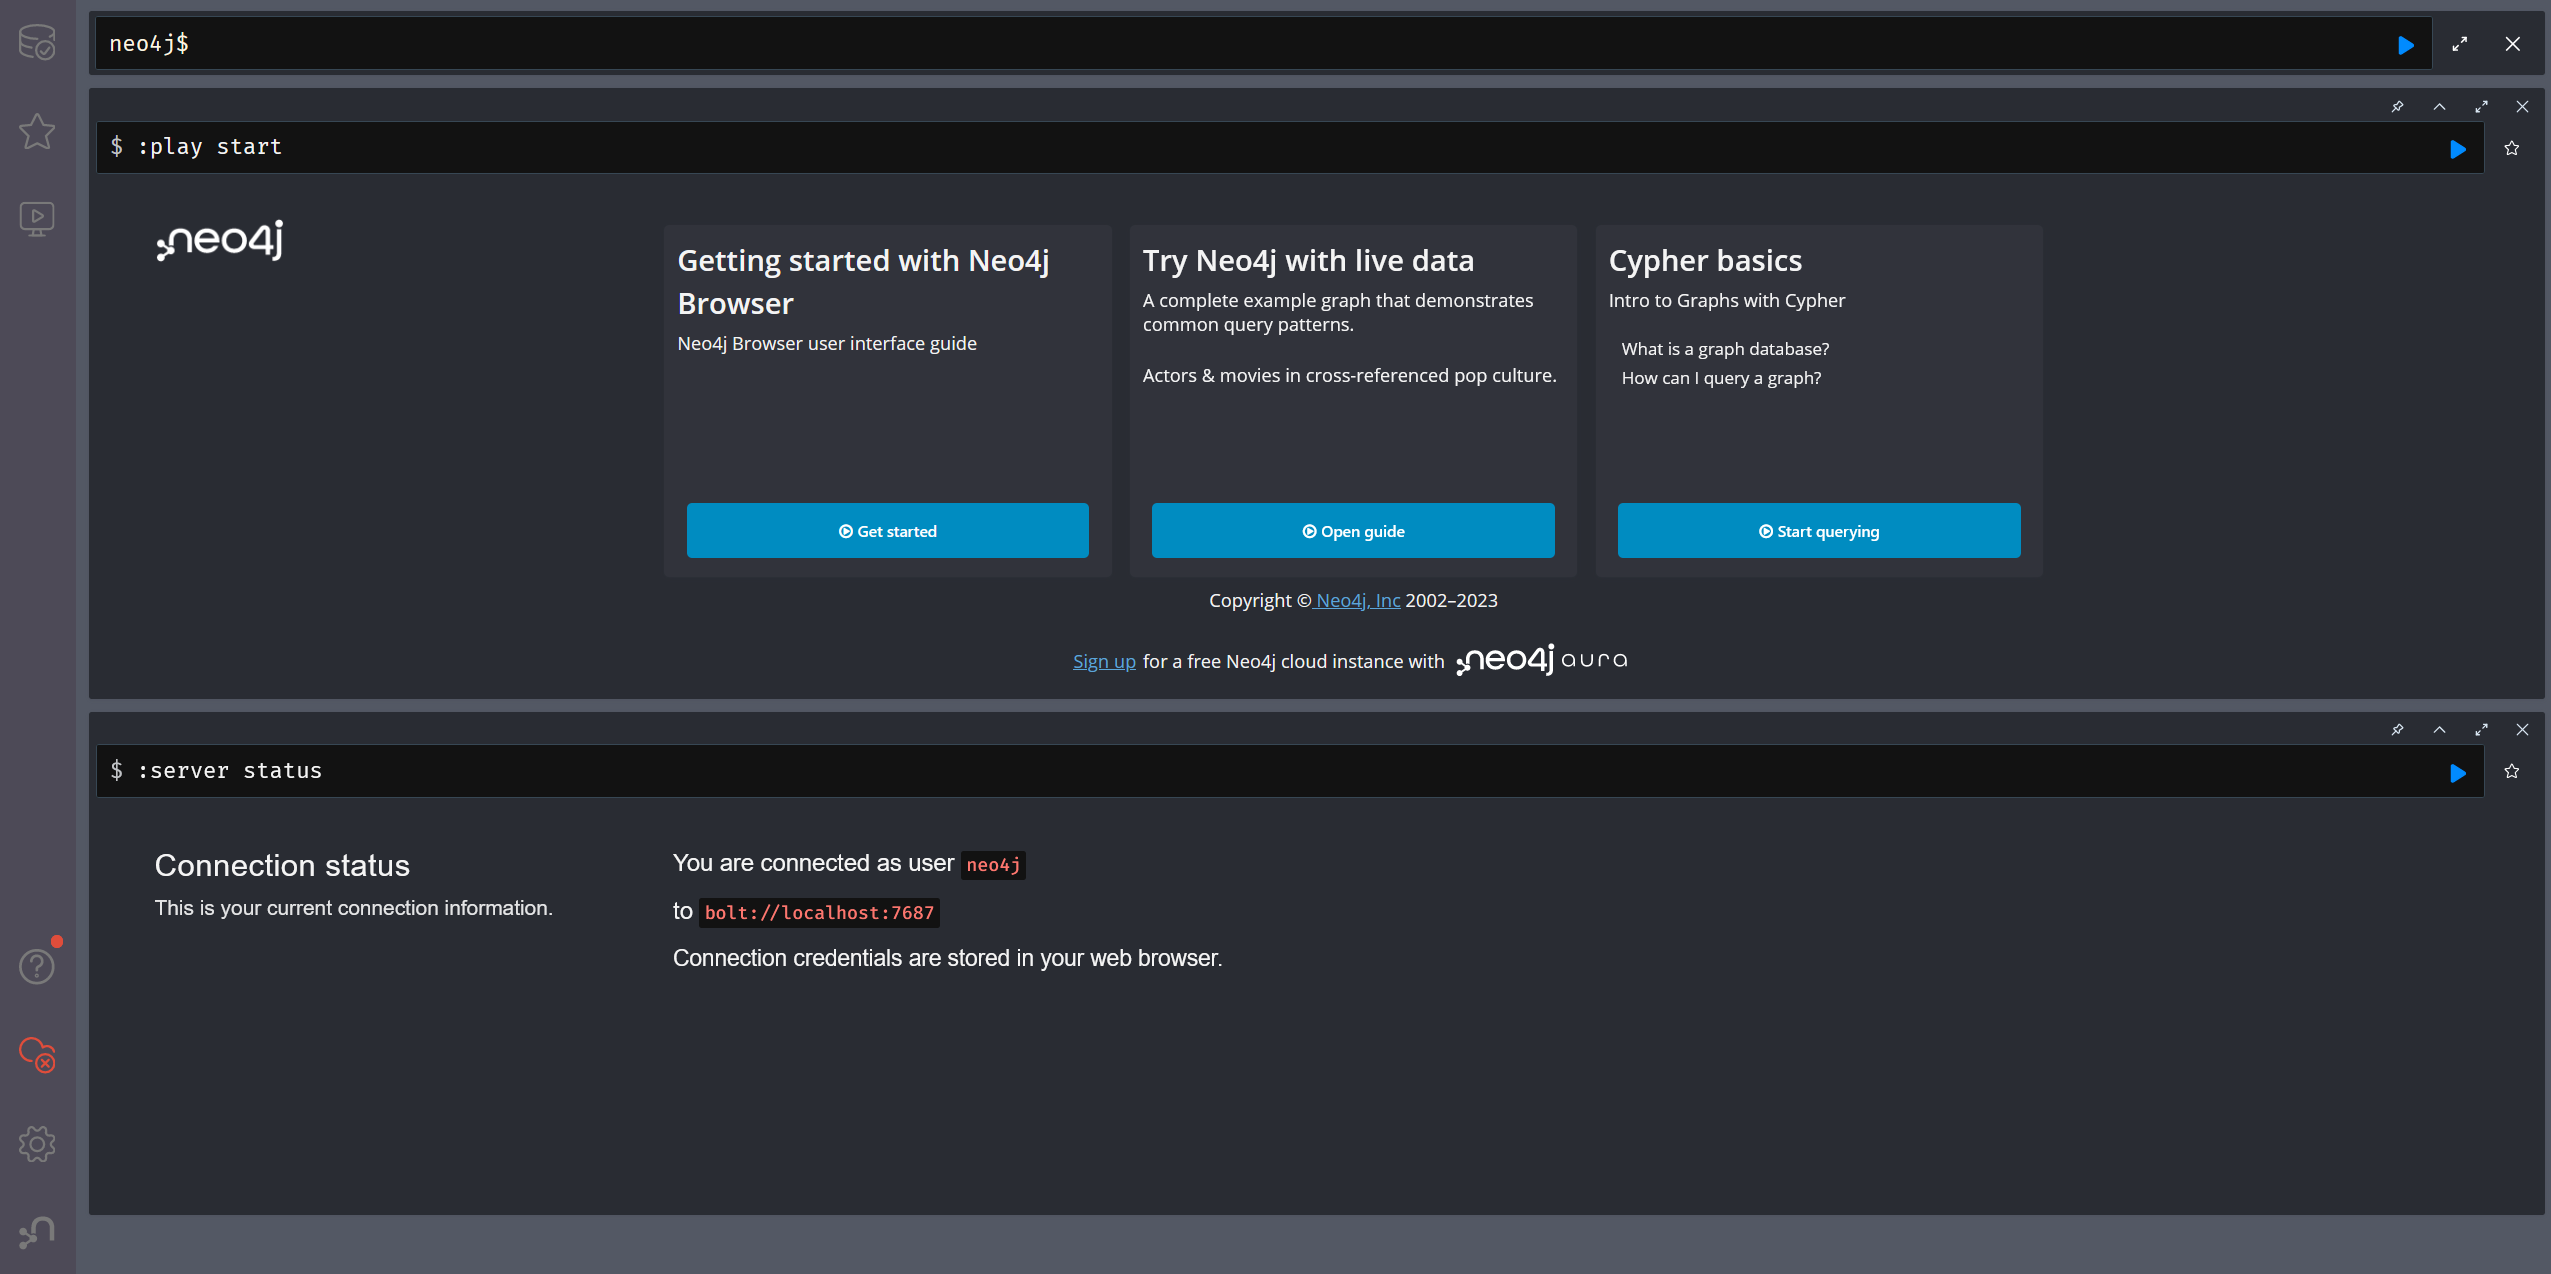
\includegraphics[width=0.8\textwidth]{images/neo4j-web-interface.png}
    \caption{Neo4j web interface}
    \label{fig:neo4j-web-interface}
\end{figure}

In general the Neo4j Docker image is an easy and fast way to get started with
Neo4j. It is our recommendation to use the Docker image for testing and
development \parencite{neo4j:docker}.

\subsection{Use case example}
In this section a use case example will be shown. The example describes simple
the relationship between professors, students, and subjects.
\subsubsection{SQL Tables}
To get a better understanding of the Neo4j data model SQL tables will be used as
the basis for the example. The following SQL tables are used:

\texttt{professor}, \texttt{student}, \texttt{subject},
\texttt{professor\_subject} and \texttt{student\_subject}.
\begin{table}[ht]
    \centering
    \subfloat[Table students]{
        \begin{tabular}{|l|l|}
            \hline
            \textbf{Student ID} & \textbf{Student name} \\
            \hline
            0                   & Tim                   \\
            1                   & Bob                   \\
            2                   & Anja                  \\
            \hline
        \end{tabular}
    }
    \quad
    \subfloat[Table professors]{
        \begin{tabular}{|l|l|}
            \hline
            \textbf{Professor ID} & \textbf{Professor name} \\
            \hline
            0                     & Müller                  \\
            1                     & Mayer                   \\
            2                     & Völlinger               \\
            \hline
        \end{tabular}
    }
    \quad
    \subfloat[Table student-subject]{
        \begin{tabular}{|l|l|}
            \hline
            \textbf{Student ID} & \textbf{Subject ID} \\
            \hline
            0                   & 2                   \\
            1                   & 1                   \\
            1                   & 2                   \\
            2                   & 0                   \\
            2                   & 3                   \\
            \hline
        \end{tabular}
    }
    \quad
    \subfloat[Table professor-subject]{
        \begin{tabular}{|l|l|l|}
            \hline
            \textbf{Subject ID} & \textbf{Subject name} & \textbf{Professor ID} \\
            \hline
            0                   & WebDev                & 0                     \\
            1                   & ICC                   & 1                     \\
            2                   & AWS                   & 2                     \\
            3                   & English               & 2                     \\
            \hline
        \end{tabular}
    }
    \caption{SQL tables}
    \label{tab:sql-tables-students}
\end{table}

The \texttt{professor\_subject} and \texttt{student\_subject} tables are
junction tables to connect the professors and students with the subjects. Even
with this simple example it is already not easily possible to read the relations
between the tables. For example if you want to know which student is taught by
which professor you have to use at least three tables to get this information.

\subsubsection{Neo4j}
In comparison to the SQL tables the Neo4j data model is much easier to read.
Relationships are directly visible and the direction of the relationship is
clear. The following image \autoref{fig:neo4j-data-model} shows the
example data in the Neo4j web interface.

\begin{figure}[ht]
    \centering
    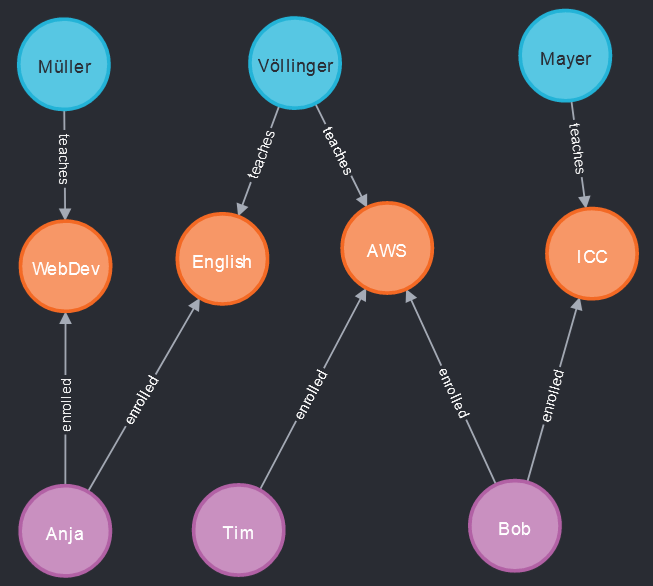
\includegraphics[width=0.8\textwidth]{images/neo4j-data-model.png}
    \caption{Neo4j data model}
    \label{fig:neo4j-data-model}
\end{figure}